\documentclass[6pt]{AiTex}
\usepackage{csvsimple}

\title{Memoria entrega 0}
\author{A.L.K.}
\date{Febrero 2024}

\begin{document}
%\datos{facultad}{universidad}{grado}{asignatura}{subtitulo}{autor}{curso}
\datos{Informática}{Universidad Complutense de Madrid}{Ingeniería informática}{Aprendizaje Automatico y Big Data}{Entrega 0: iteración vs vectorización}{Alejandro Barrachina Argudo}{2023-2024}
% \portadaApuntes
% \pagestyle{empty}
% \tableofcontents
% \pagestyle{empty}
\justify

\begin{center}

    {\huge \textbf{\underline{\subtitulo}}} \\
    { \lesson - \autor}

\end{center}


\section*{Introducción}

En este documento se explicará el código del entregable 0 y la diferencia entre vectorización e iteración.

Para esta práctica se usarán los siguientes \textit{imports} vistos en la figura \ref{fig:imports}. Para ver las diferencias de eficiencia entre vectorización e iteración usaremos el cálculo de la integral por el método de montecarlo.
\begin{figure}[H]
    \centering
    \lstinputlisting[firstline=1,lastline=7, style=custompython]{../Entregable0.py}
    \caption{Código de las bibliotecas usadas}
    \label{fig:imports}
\end{figure}

\section{Iteración}

En la parte iterativa del problema usaremos las funciones estándar de bucle de python y listas intensionales.

La función \textcolor{codepurple}{calc\_max\_func} (\ref{fig:calc_max_func}) nos da el máximo valor que alcanza la función haciendo un muestreo uniforme del intervalo $[a,b]$, este máximo será el que usaremos para generar los puntos aleatorios para el algoritmo de montecarlo.
Tras conseguir el máximo, la función \textcolor{codepurple}{integra\_mc\_iter} (\ref{fig:integra_mc_iter}) genera los puntos aleatorios y compara con la función para ver si el punto está por encima o por debajo. Luego usamos la fórmula $\frac{num\;debajo}{num\;total}(b-a)M$ para calcular el area aproximada de la integral.

Podemos ver que este método es bastante lento cuando empezamos a tener un mayor número de puntos.

\begin{figure}[H]
    \centering
    \lstinputlisting[firstline=77,lastline=98, style=custompython]{../Entregable0.py}
    \caption{Código de la función calc\_max\_func}
    \label{fig:calc_max_func}
\end{figure}

\begin{figure}[H]
    \centering
    \lstinputlisting[firstline=51,lastline=75, style=custompython]{../Entregable0.py}
    \caption{Código de la función integra\_mc\_iter}
    \label{fig:integra_mc_iter}
\end{figure}

\section{Vectorizado}

Para la vectorización usamos la librería \textit{numpy} y simplificamos todo el código a una sola función \textcolor{codepurple}{integra\_mc\_vect} (\ref{fig:integra_mc_vect}). La función \textcolor{codepurple}{np.vectorize()} nos permite que cualquier función se pueda aplicar a vectores, simplificando así la computación de la función. con \textcolor{codepurple}{np.linspace()} generamos una distribución de puntos en el eje x a los que aplicarles la función vectorizada, tras esto usamos \textcolor{codepurple}{np.max()} para hallar el máximo valor que alcanza la función.

Con \textcolor{codepurple}{np.random.uniform} generamos un vector de valores de la función desde 0 hasta el máximo, con esto y los primeros valores generados de y podemos ver que puntos quedan por arriba y cuales por debajo de la función. Con esto y la fórmula anterior, volvemos a calcular la integral aproximada de la función.

\begin{figure}[H]
    \centering
    \lstinputlisting[firstline=24,lastline=49, style=custompython]{../Entregable0.py}
    \caption{Código de la función integra\_mc\_vect}
    \label{fig:integra_mc_vect}
\end{figure}

\section{Funciones y generación de datos}

En esta sección se explican otras funciones que se han usado en el programa pero que no afectan a la métrica o las propias funciones que se usan para probar la integral.

\subsection{Pruebas}
Para las pruebas tenemos dos funciones, una que generará los test (\ref{fig:test_cases}) y otra que correrá cada test individual cinco veces para sacar una media (\ref{fig:test_increment}).

La función \textcolor{codepurple}{test\_cases} se encarga de generar un vector de tiempos (tanto vectoriales como iterativos) conseguidos de cada caso de prueba, también genera dichos casos de prueba (con una función de \textit{numpy}). Esta función también se encarga de dibujar los gráficos de tiempo de los casos de prueba.

La función \textcolor{codepurple}{test\_increment} se encarga de coger un caso (número de puntos) y correrlo cinco veces de manera vectorizada e iterativa, midiendo sus tiempos y haciendo la media de todas las ejecuciones. También nos muestra por pantalla el valor conseguido para asegurarnos de que es un valor correcto y guarda dichos datos en un csv para exportarlos más fácilmente a documentos (como este) o para su estudio posterior.

En la función \textcolor{codepurple}{test\_cases} generamos un pequeño gráfico de cada función probada para ver que es la que queremos calcular realmente, para ello usamos la función \textcolor{codepurple}{gen\_fun\_graph} (\ref{fig:gen_fun_graph}).

\begin{figure}[H]
    \centering
    \lstinputlisting[firstline=191,lastline=231, style=custompython]{../Entregable0.py}
    \caption{Código de la función test\_cases}
    \label{fig:test_cases}
\end{figure}

\begin{figure}[H]
    \centering
    \lstinputlisting[firstline=124,lastline=163, style=custompython]{../Entregable0.py}
    \caption{Código de la función test\_increment}
    \label{fig:test_increment}
\end{figure}

\begin{figure}[H]
    \centering
    \lstinputlisting[firstline=167,lastline=188, style=custompython]{../Entregable0.py}
    \caption{Código de la función gen\_fun\_graph}
    \label{fig:gen_fun_graph}
\end{figure}

\subsection{Funciones probadas}

Las funciones probadas han sido el \textcolor{codepurple}{cuadrado} de un número (\ref{fig:cuadrado}), la función \textcolor{codepurple}{sin} de la biblioteca \textit{math} y \textcolor{codepurple}{fun2} (\ref{fig:fun2}), una función simplona porque no se me ocurría otra cosa. Las visualizaciones de dichas funciones se pueden ver en las figuras \ref{fig:fun_cuadrado}, \ref{fig:fun_seno} y \ref{fig:fun_fun2} respectivamente

\begin{figure}[H]
    \centering
    \lstinputlisting[firstline=100,lastline=109, style=custompython]{../Entregable0.py}
    \caption{Código de la función cuadrado}
    \label{fig:cuadrado}
\end{figure}

\begin{figure}[H]
    \centering
    \lstinputlisting[firstline=112,lastline=121, style=custompython]{../Entregable0.py}
    \caption{Código de la función fun2}
    \label{fig:fun2}
\end{figure}

\begin{figure}[H]
    \centering
    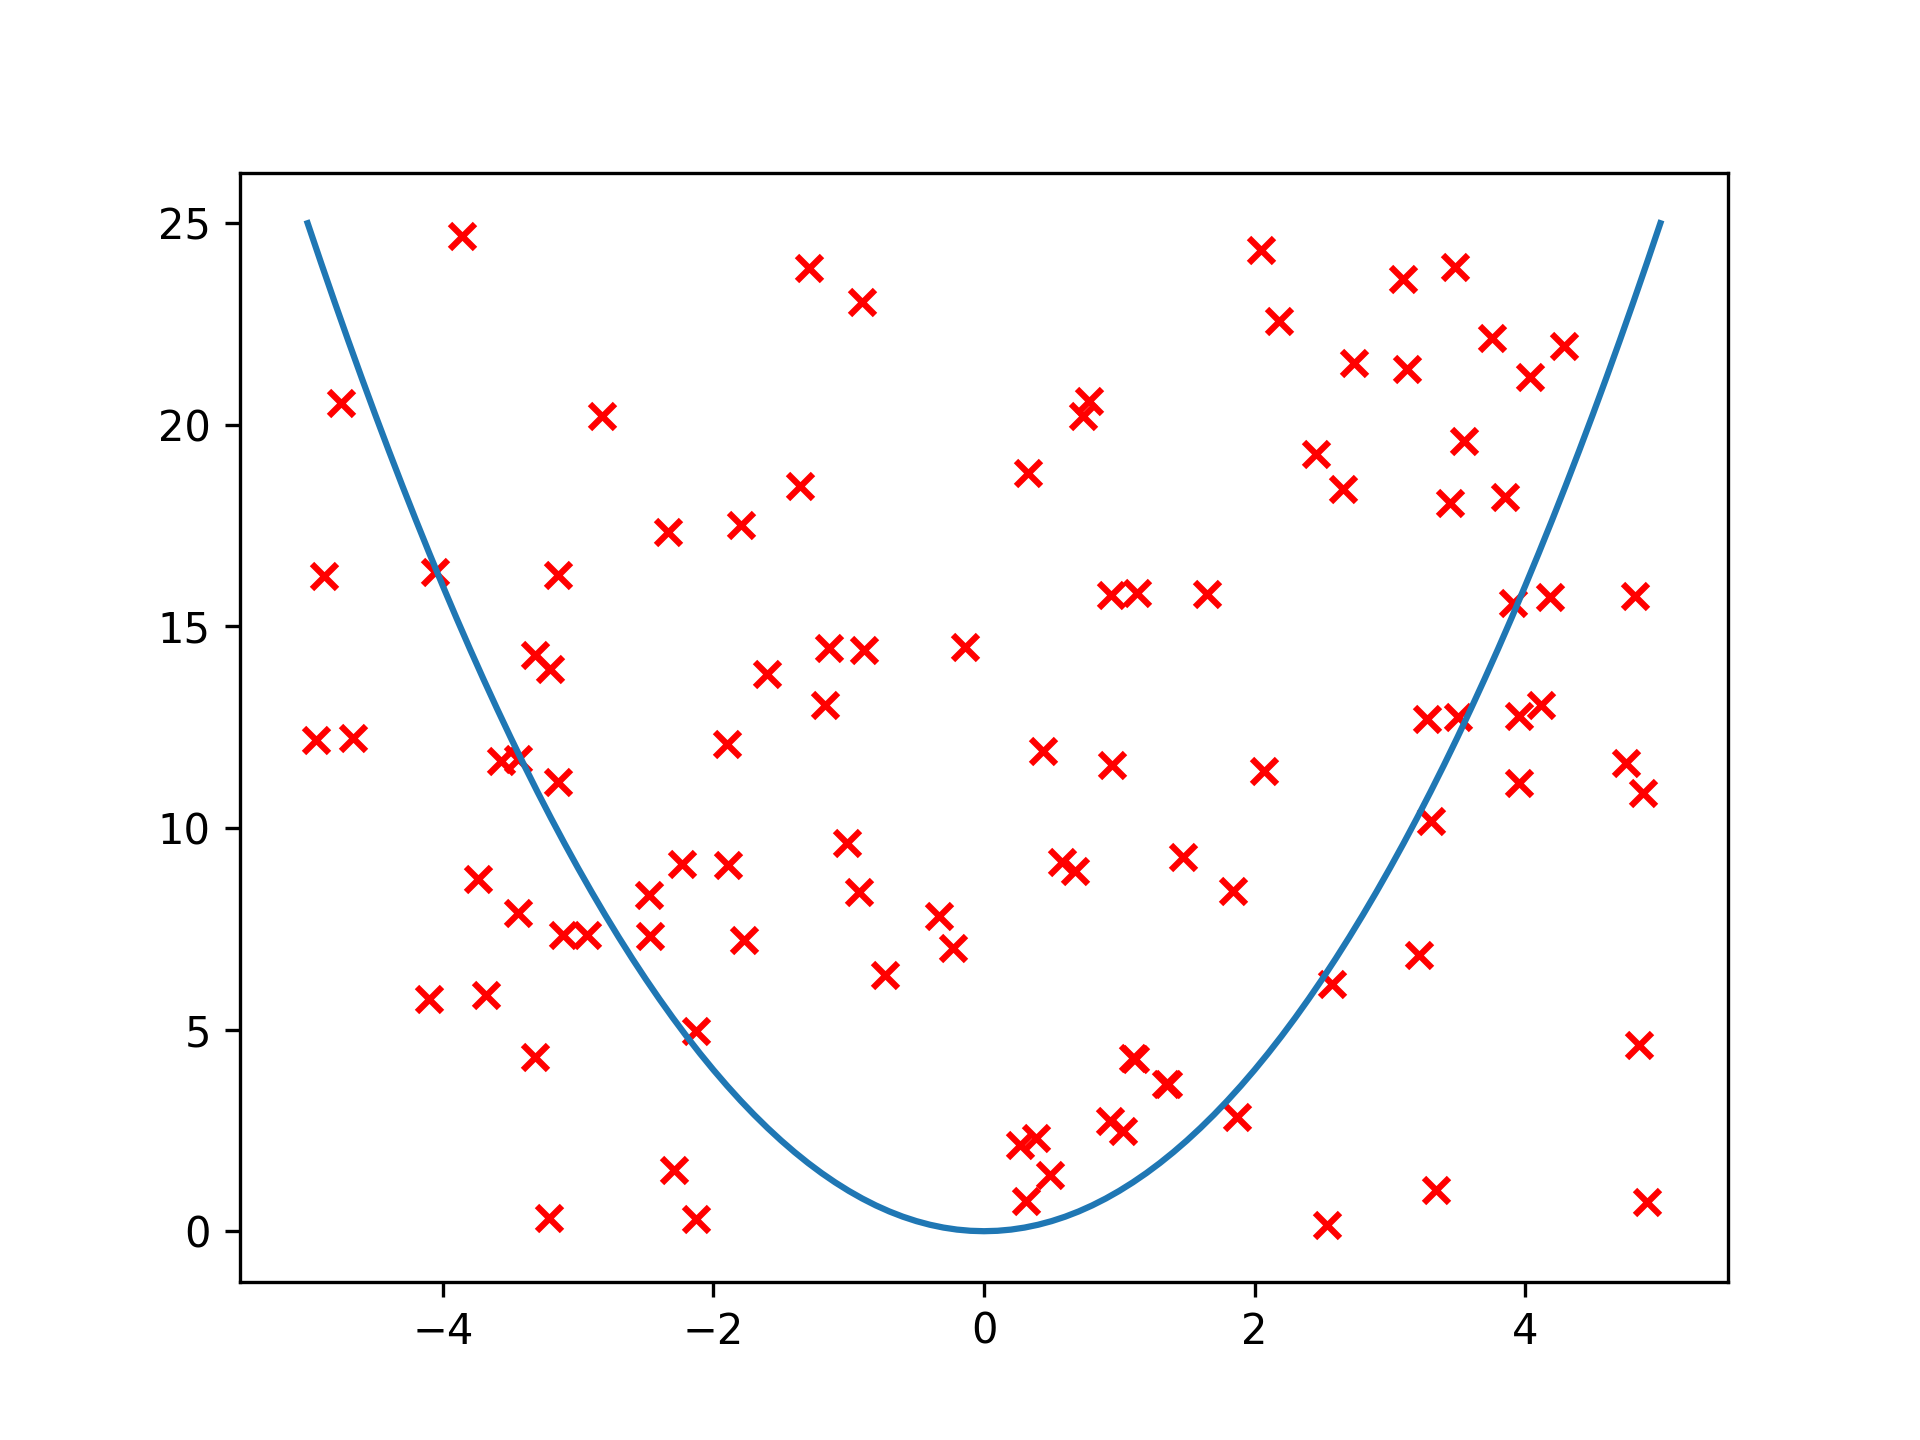
\includegraphics[width=0.8\textwidth]{./imagenes/cuadrado.png}
    \caption{Gráfico de la función cuadrado}
    \label{fig:fun_cuadrado}
\end{figure}

\begin{figure}[H]
    \centering
    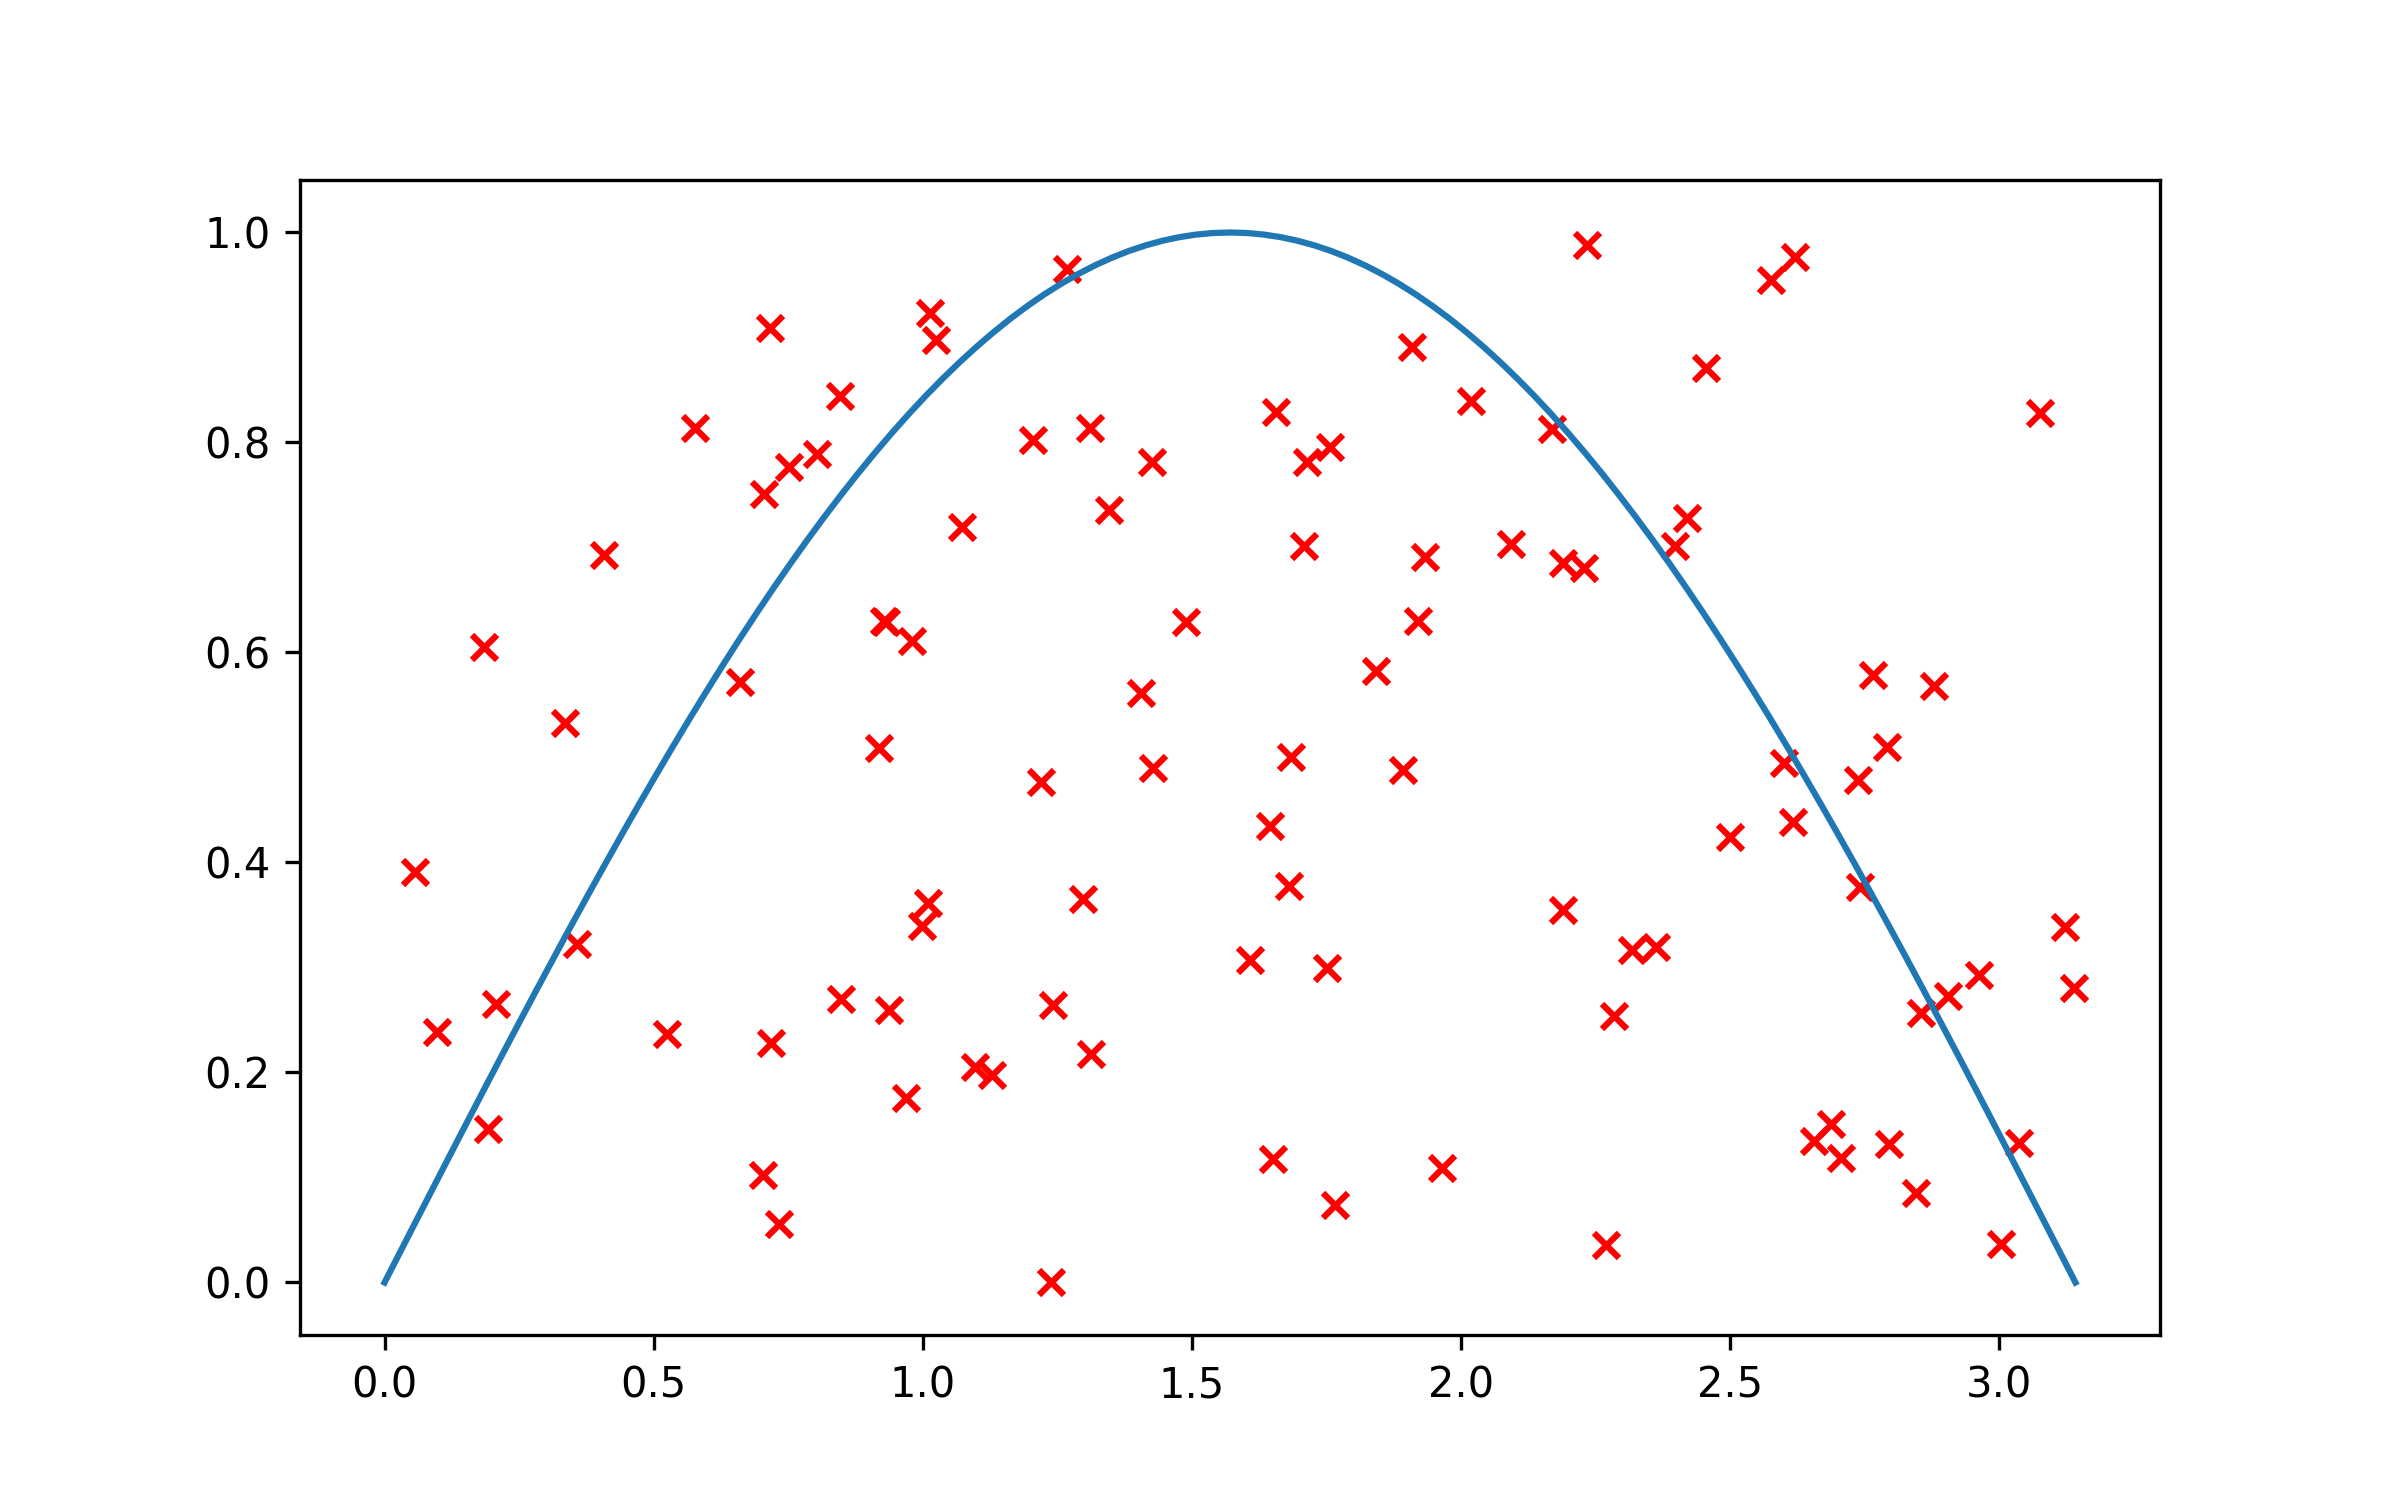
\includegraphics[width=0.8\textwidth]{./imagenes/sin.png}
    \caption{Gráfico de la función sin}
    \label{fig:fun_seno}
\end{figure}

\begin{figure}[H]
    \centering
    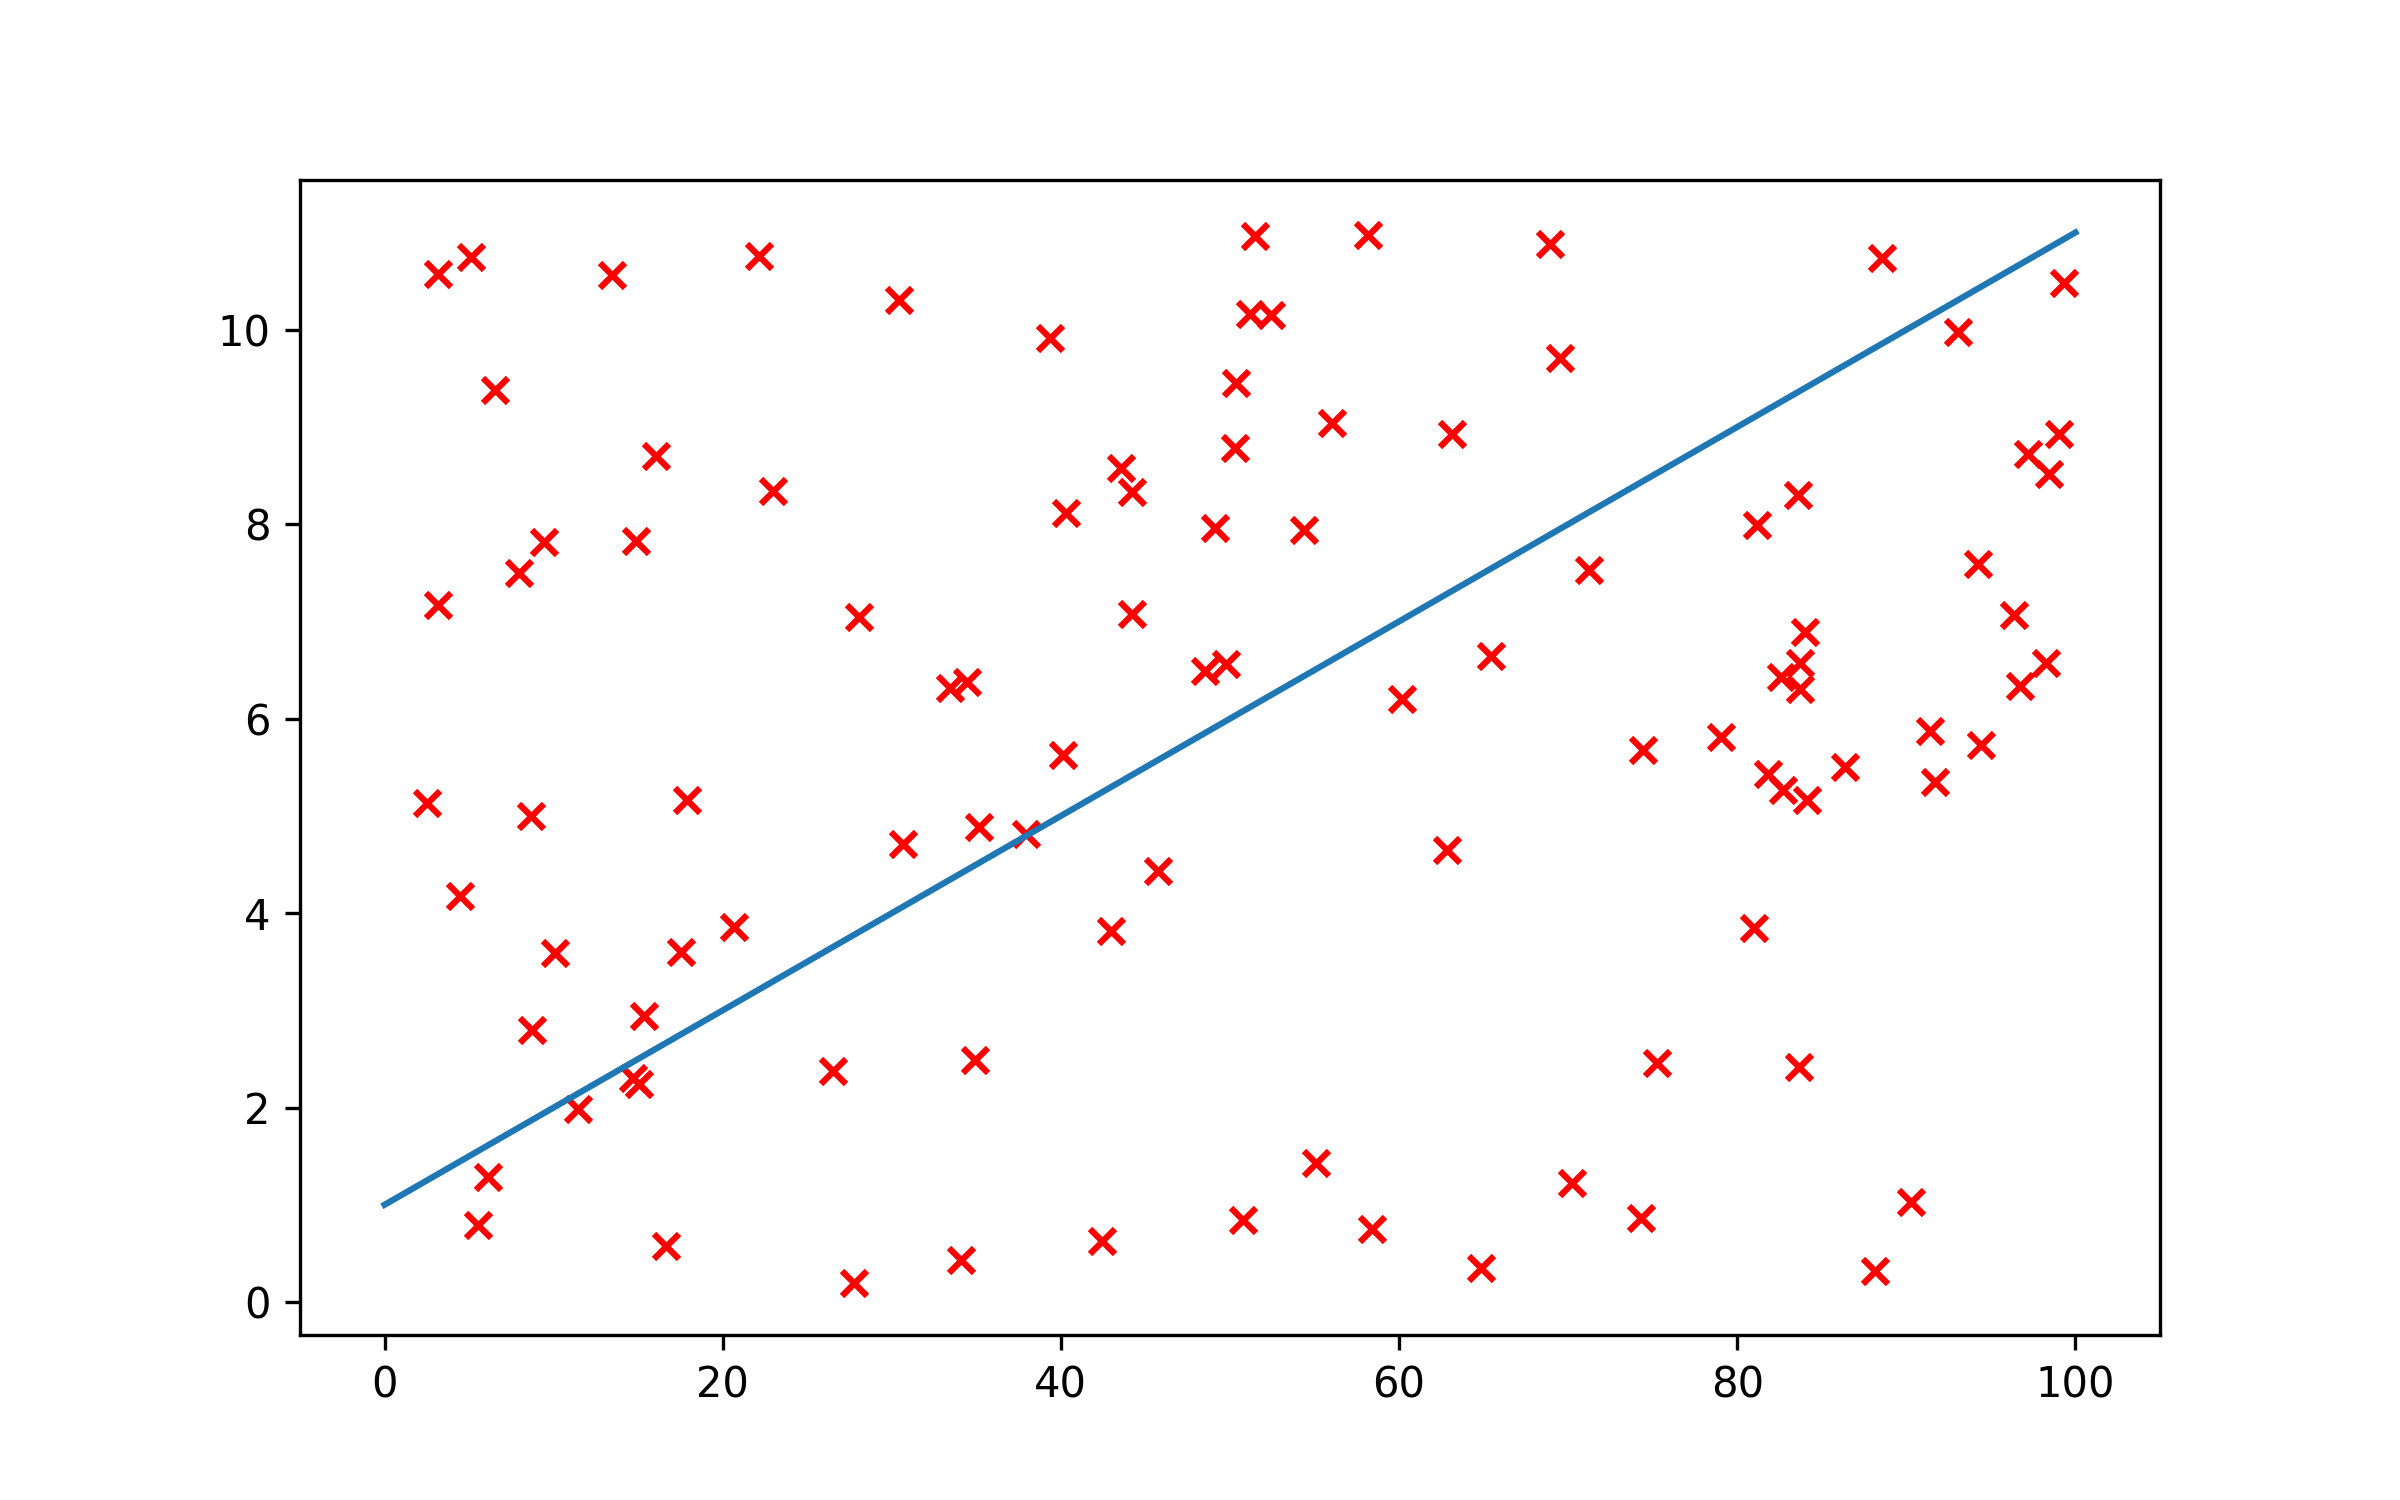
\includegraphics[width=0.8\textwidth]{./imagenes/fun2.png}
    \caption{Gráfico de la función fun2}
    \label{fig:fun_fun2}
\end{figure}

\section{conclusiones}

Viendo los tiempos en las tablas \ref{table:cuadrado}, \ref{table:sin}, \ref{table:fun2} y en las figuras \ref{fig:tiempos_cuadrado}, \ref{fig:tiempos_sin} y \ref{fig:tiempos_fun2}, la vectorización apenas crece en tiempo cuando aumentamos los puntos en comparación con las funciones iterativas. Esto muestra bastante bien que las funciones de \textit{numpy} van a ser muy útiles a la hora de tratar con grandes números de datos.

\begin{table}[H]
    \centering
    \csvreader[tabular=|c|r|r|,
        table head=\hline \textbf{Número puntos} & \textbf{ Tiempo Iterativo(ms)} & \textbf{Tiempo Vectorizado (ms)}\\ \hline,
        late after line=\\ \hline]
    {./recursos/cuadrado.csv}{1=\casos,2=\iterativo,3=\vectorizado}
    {\casos & \iterativo & \vectorizado}
    \caption{Comparación de tiempos de ejecución en la función cuadrado}
    \label{table:cuadrado}
\end{table}

\begin{figure}[H]
    \centering
    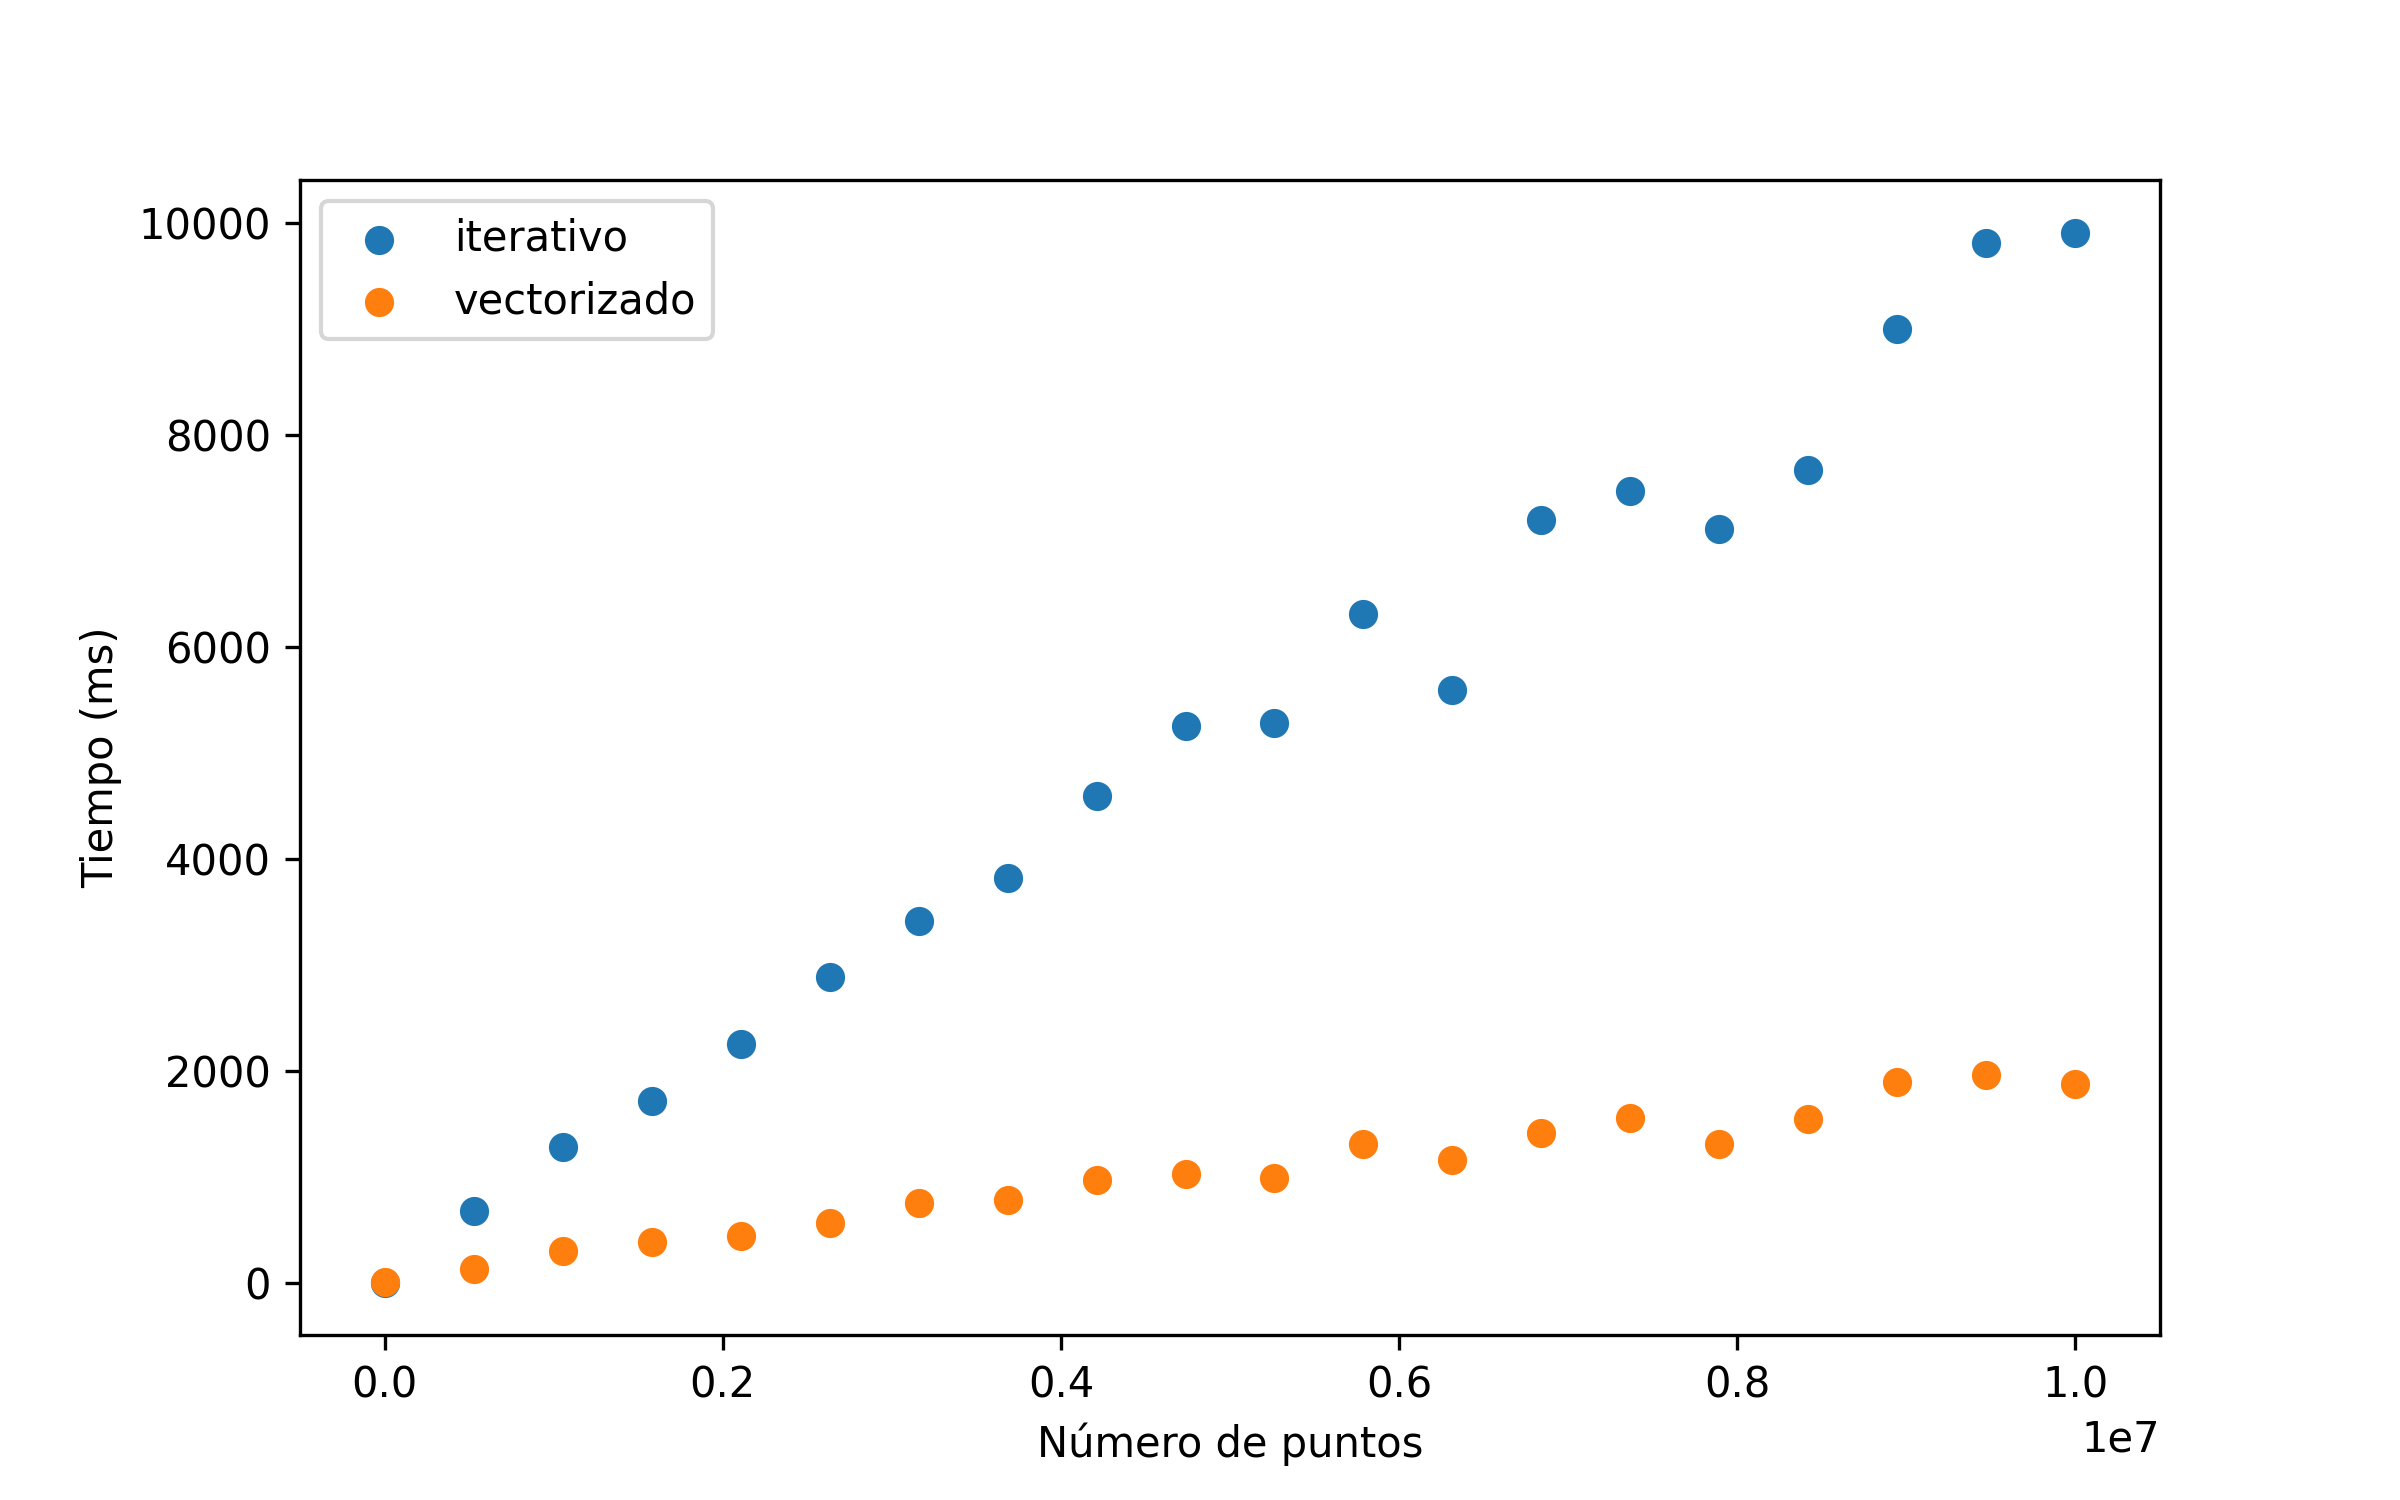
\includegraphics[width=0.7\textwidth]{./imagenes/tiempos_cuadrado.png}
    \caption{Gráfica de tiempo de la función cuadrado}
    \label{fig:tiempos_cuadrado}
\end{figure}

\begin{table}[H]
    \centering
    \csvreader[tabular=|c|r|r|,
        table head=\hline \textbf{Número puntos} & \textbf{ Tiempo Iterativo(ms)} & \textbf{Tiempo Vectorizado (ms)}\\ \hline,
        late after line=\\ \hline]
    {./recursos/sin.csv}{1=\casos,2=\iterativo,3=\vectorizado}
    {\casos & \iterativo & \vectorizado}
    \caption{Comparación de tiempos de ejecución en la función sin}
    \label{table:sin}
\end{table}

\begin{figure}[H]
    \centering
    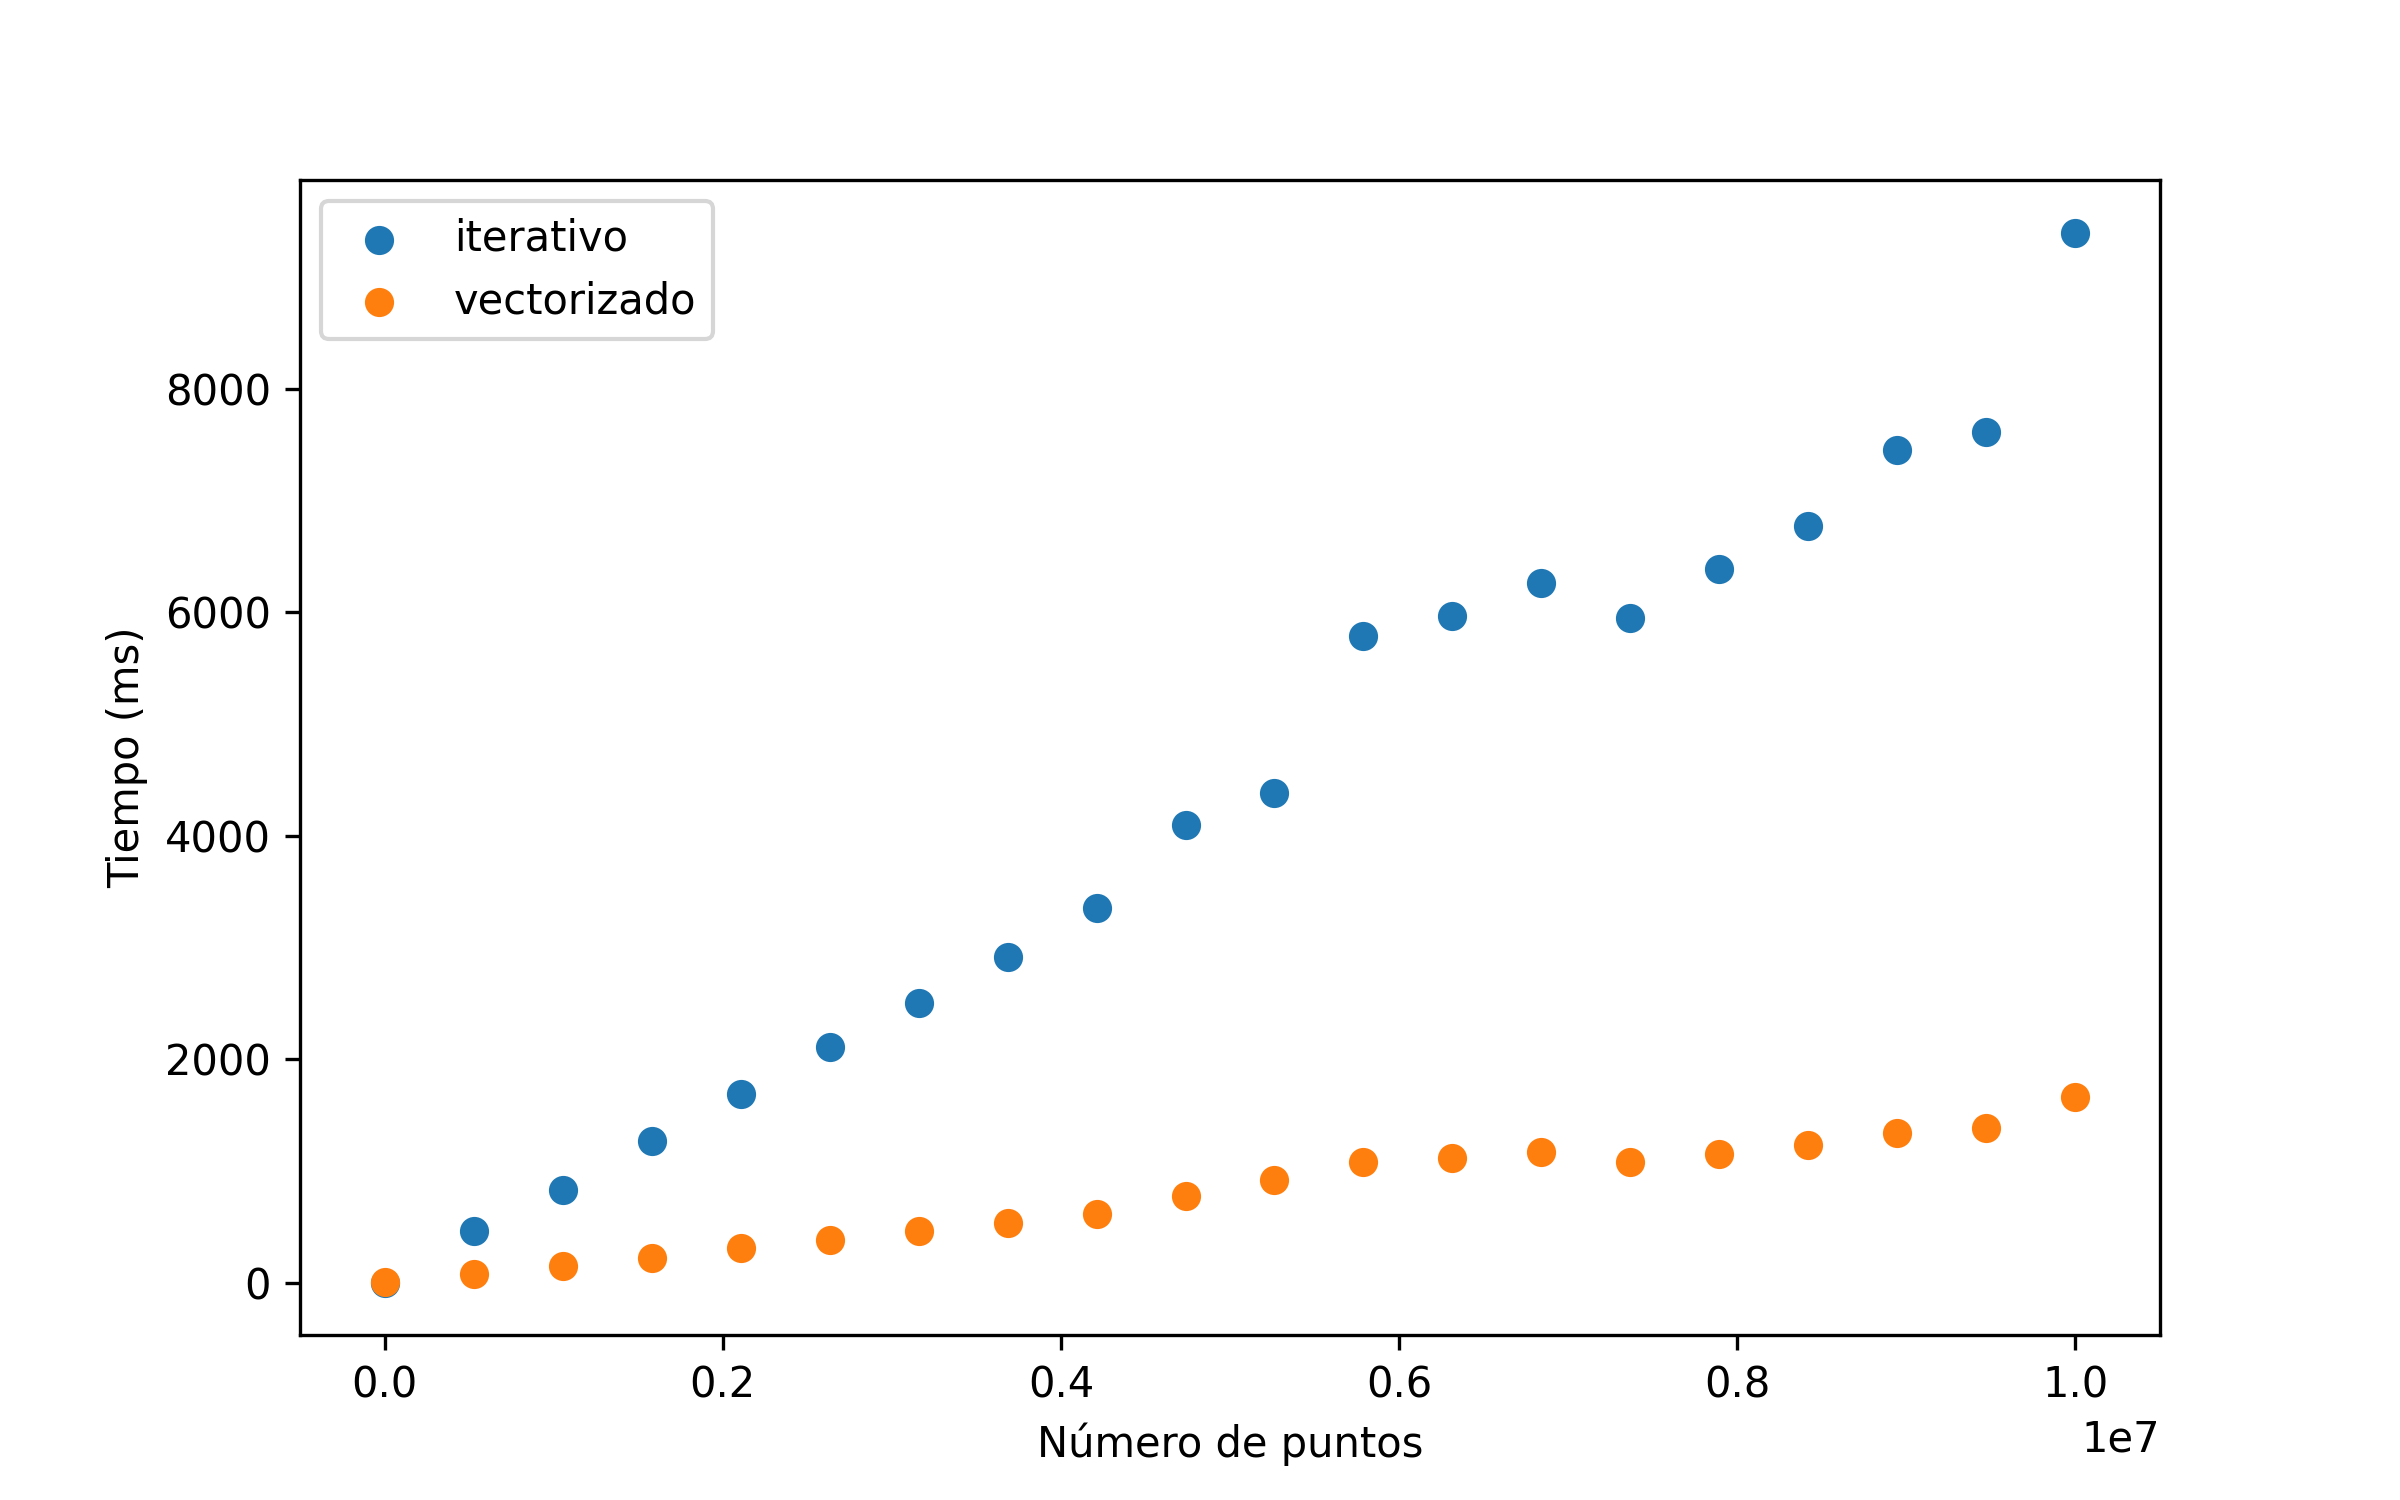
\includegraphics[width=0.7\textwidth]{./imagenes/tiempos_sin.png}
    \caption{Gráfica de tiempo de la función sin}
    \label{fig:tiempos_sin}
\end{figure}

\begin{table}[H]
    \centering
    \csvreader[tabular=|c|r|r|,
        table head=\hline \textbf{Número puntos} & \textbf{ Tiempo Iterativo(ms)} & \textbf{Tiempo Vectorizado (ms)}\\ \hline,
        late after line=\\ \hline]
    {./recursos/fun2.csv}{1=\casos,2=\iterativo,3=\vectorizado}
    {\casos & \iterativo & \vectorizado}
    \caption{Comparación de tiempos de ejecución en la función 'fun2'}
    \label{table:fun2}
\end{table}

\begin{figure}[H]
    \centering
    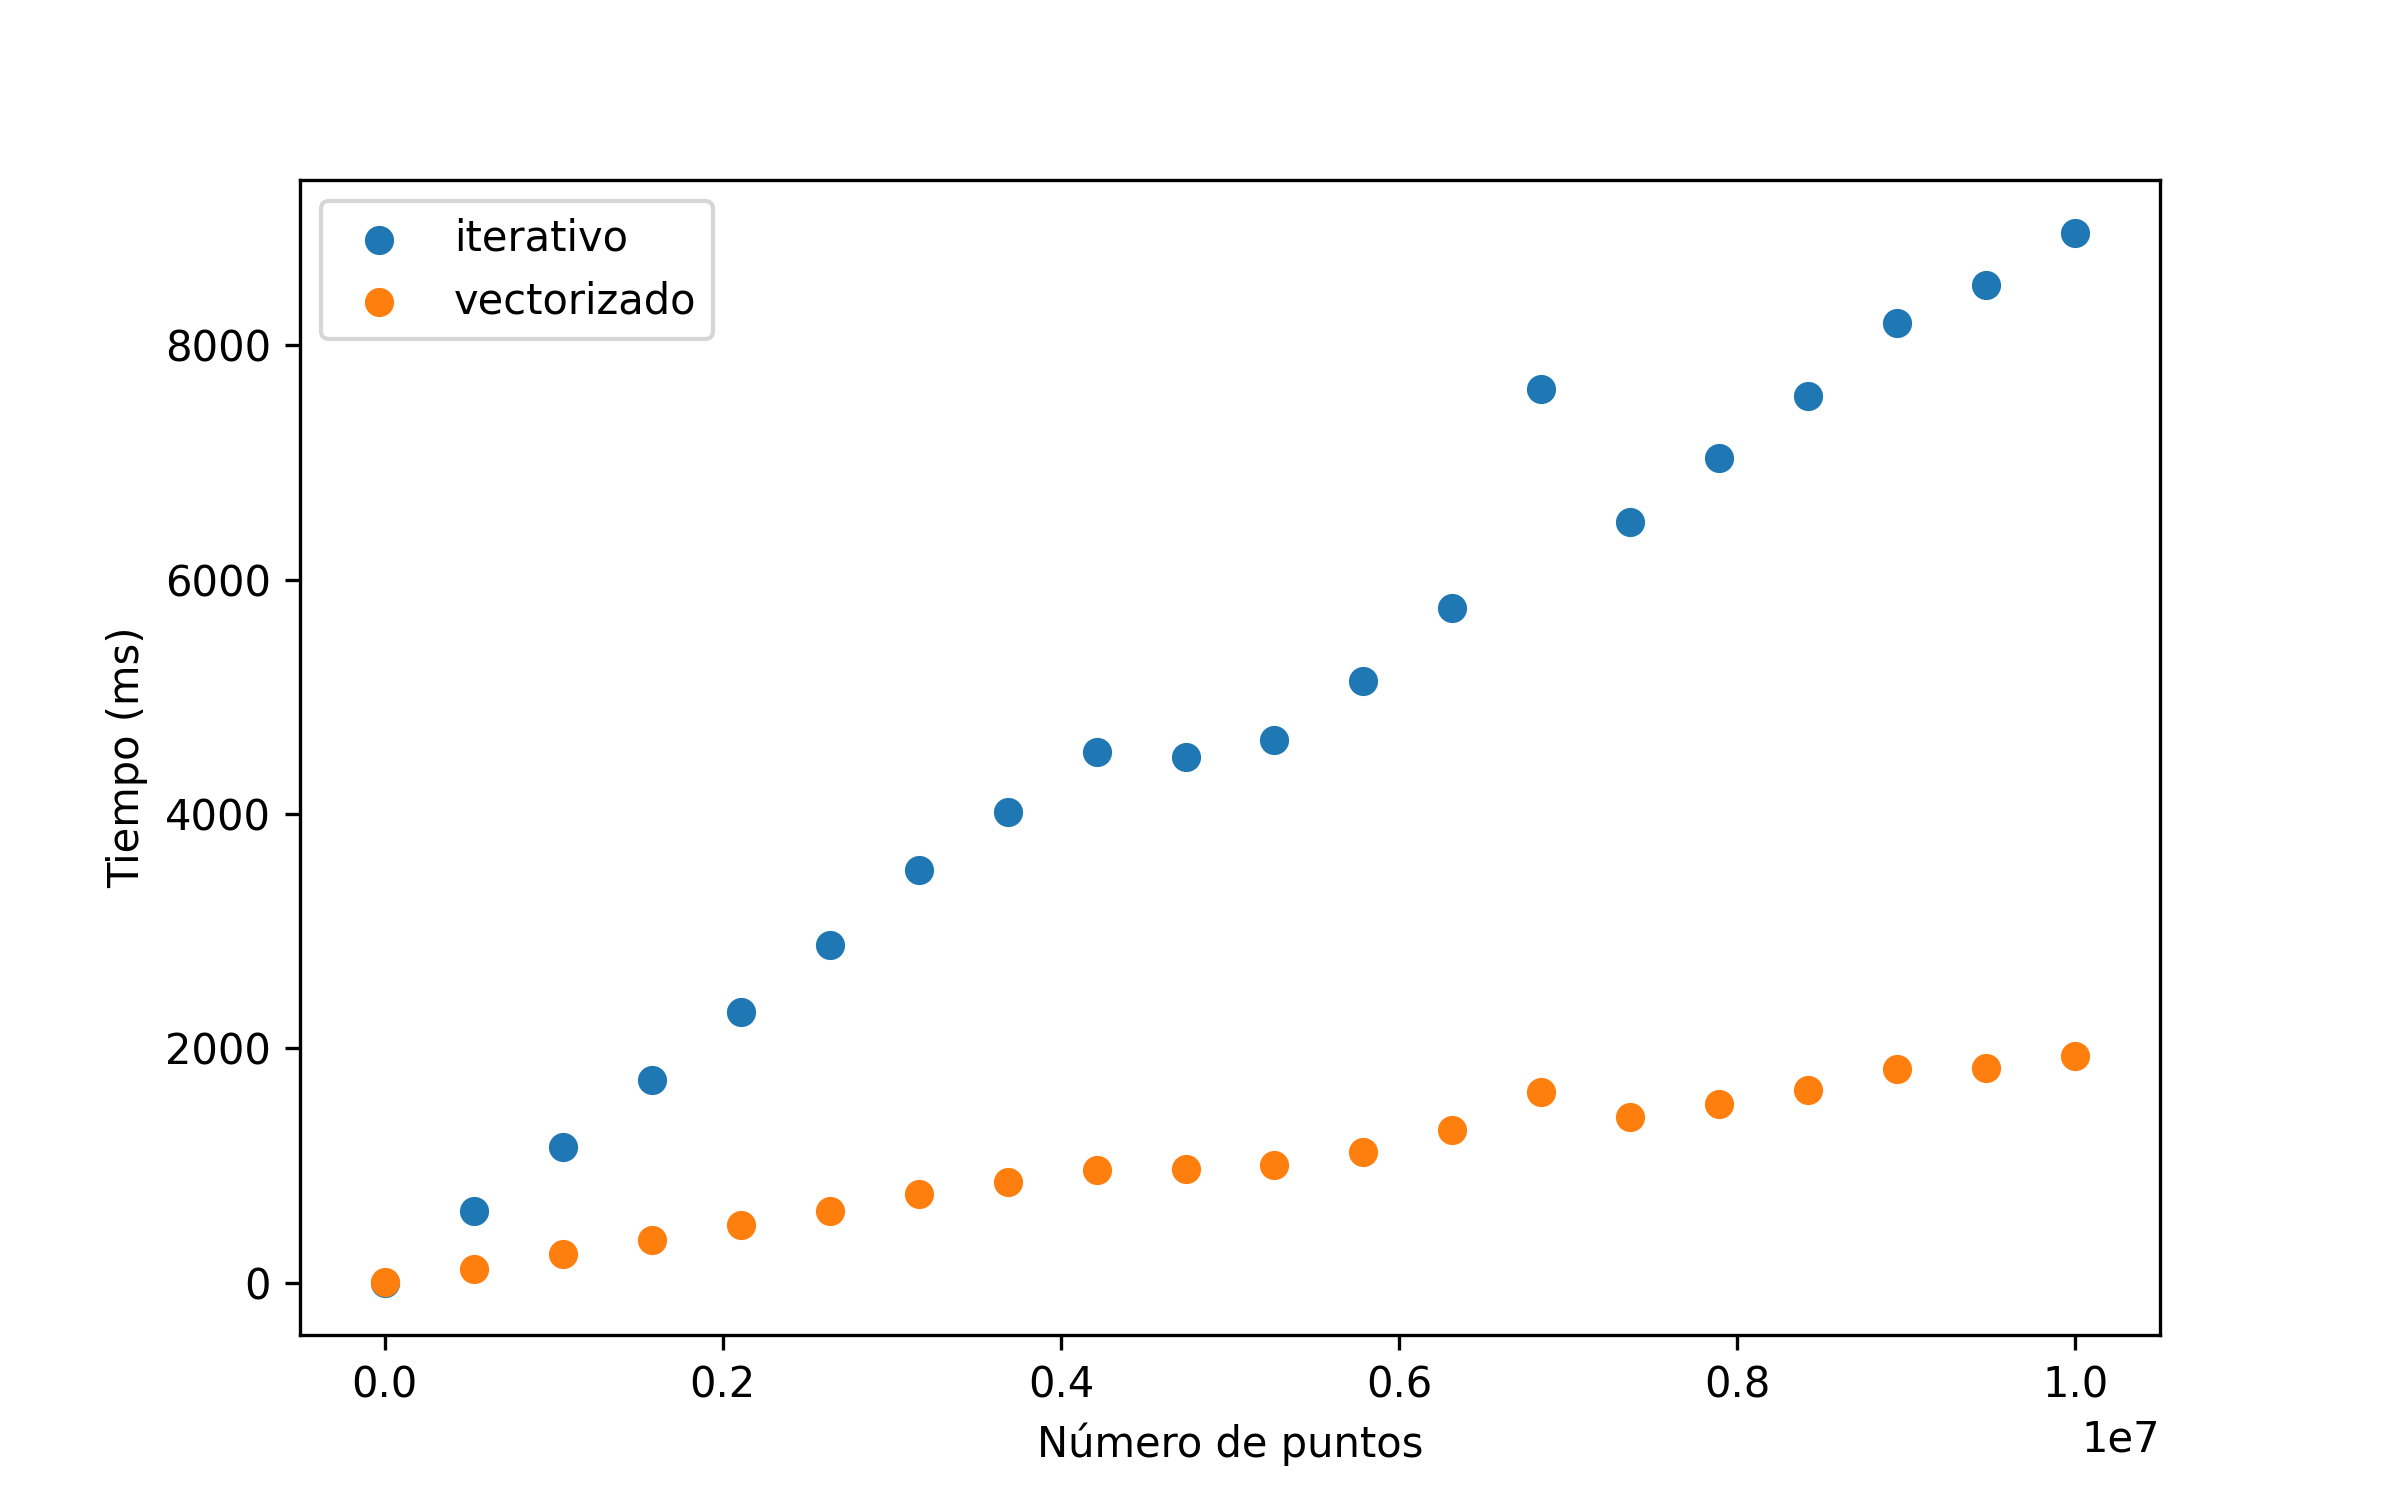
\includegraphics[width=0.7\textwidth]{./imagenes/tiempos_fun2.png}
    \caption{Gráfica de tiempo de la función fun2}
    \label{fig:tiempos_fun2}
\end{figure}



\end{document}
